\documentclass{article}
\usepackage{pgfplots}

\begin{document}

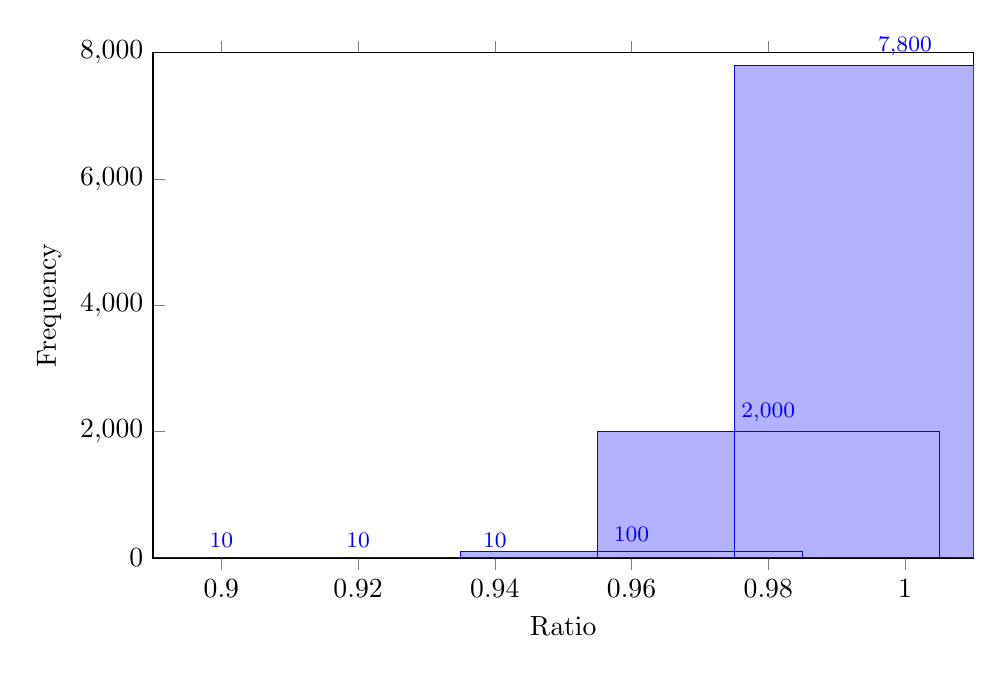
\begin{tikzpicture}
    \begin{axis}[
        width=12cm,
        height=8cm,
        xlabel={Ratio},
        ylabel={Frequency},
        xtick={0.9, 0.92, 0.94, 0.96, 0.98, 1},
        ybar,
        bar width=0.05,
        ymin=0,
        ymax=8000,
        nodes near coords,
        every node near coord/.append style={font=\footnotesize},
        ]
        \addplot coordinates {
            (0.9, 10)
            (0.92, 10)
            (0.94, 10)
            (0.96, 100)
            (0.98, 2000)
            (1, 7800)
        };
    \end{axis}
\end{tikzpicture}

\end{document}